\paragraph{Ausgangssignale}
Es wurden insgesamt vier unterschiedliche Aufnahmen als Testsignale herangezogen. Dabei wurden auch zwei Aufnahmen im B-Format synthetisch erzeugt, um auch sehr gerichtete Signale vergleichen zu können:

\begin{itemize}
	\item Synthetisches Zirpen, rotierend in Azimuth
	\item Synthetisches Zirpen, rotierend in Azimuth, nachträglich verhallt mittels FDN-Plugin
	\item Live-Musik Aufnahme
	\item Umgebungsgeräusche Straßenkreuzung
\end{itemize}

Die synthetischen Signale wurden dabei mit Hilfe eines weiteren Skriptes in Octave erzeugt. Das zusätzlich verhallte Signal wurde nachträglich in Reaper mit dem FDN Reverb Plugin aus der IEM Plugin Suite bearbeitet. Dies soll einfach einen direkteren Vergleich der Performance zwischen stark gerichtetem und stark diffusem Signal bieten. Die Live-Musik Aufnahme wurde im Cube angefertigt und bietet einen große Räumlichkeit, wobei die Ambience-Aufnahme an einer Straßenkreuzung hier die größte Diffusität aufweist. Diese Aufnahmen wurden mit Soundfield Mikrofonen durchgeführt. Somit werden im Hörversuch vier sehr unterschiedliche Aufnahmeszenarien verglichen.

\paragraph{Verglichene Kombinationen von Dekorrelation und Dekodierung}

Die folgende Liste zeigt die verglichenen Kombinationen aus Upmixing-, Dekorrelations- und Dekodierungsmethoden:

\begin{itemize}
	\item DirAC, 12 Speaker + Random Phase Decorrelation
	\item DirAC, 12 Speaker + FDN Decorrelation
	\item DirAC, T-Design + FDN Decorrelation
	\item DirAC, T-Design + Widening Plugin
	\item Harpex
	\item Compass
\end{itemize}

Abbildung ~\ref{fig_algos} ist eine schematische Darstellung der Wiedergabe der Testsignale. Die Wiedergabe ist grundsätzlich immer eine Kombination aus vorhergehender Erzeugung und Bearbeitung in einem Octave-Skript, und Wiedergabe und Bearbeitung in Reaper mittels Plugins.

\begin{figure}[!ht]
  \centering
  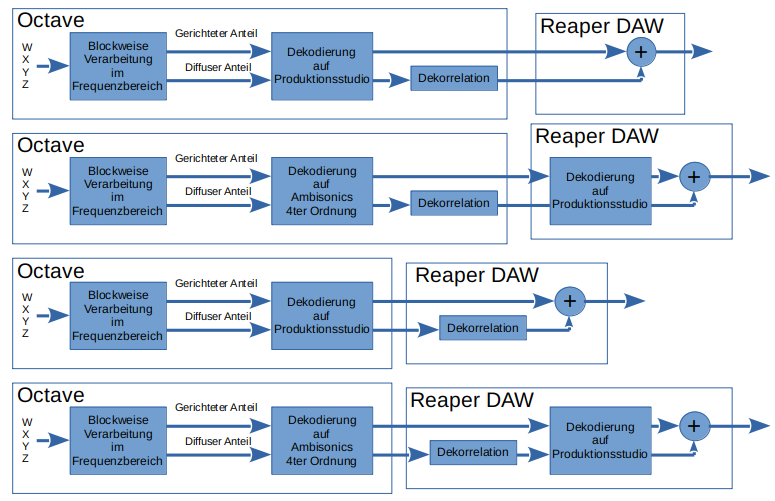
\includegraphics[width=0.9\textwidth]{aufbau/plots/algos.png}
  \label{fig:algos}
  \caption{Flussdiagram Wiedergabe im Produktionsstudio}
\end{figure}

Die Dekodierung der ambisonischen Signale passiert für alle Signale in Octave. Nach dem DirAC-Upmixing wird die Dekodierung entweder auf die 12-Speaker-Anordnung des Produktionsstudios durchgeführt, oder allgemein für ein 9-Design T-Design. Daher können die 12-Speaker-dekodierten Signale in Reaper anschließend direkt auf die Lautsprecher ausgerichtet wiedergegeben werden, und das T-Design-Signal wird zuvor noch mit einem Dekodierungsplugin auf die Lautsprecher aufgeteilt.

\paragraph{Wiedergabesystem}
Als Wiedergabesytem wurde die Lautsprecheranordnung des Produktionsstudios des IEM verwendet. Prinzipiell besteht die Lautsprecheranordnung im Produktionsstudio aus zwei Ringen in horizontaler Lage und darüber, und einem Deckenlautsprecher. Es werden insgesamt 12 Speaker verwendet, jedoch befindet sich keine Lautsprecher in vertikaler Richtung unter dem Horizont. Einer Visualisierung der Lautsprecheranordnung ist in Abb. ~\ref{fig:aufb:prod_stud} dargestellt. Der Nadir-Lautsprecher in der Abbildung ist eine imaginäre Schallquelle um Signale unter dem Horizont auf andere Lautsprecher zu verteilen.

\begin{figure}[!ht]
  \centering
  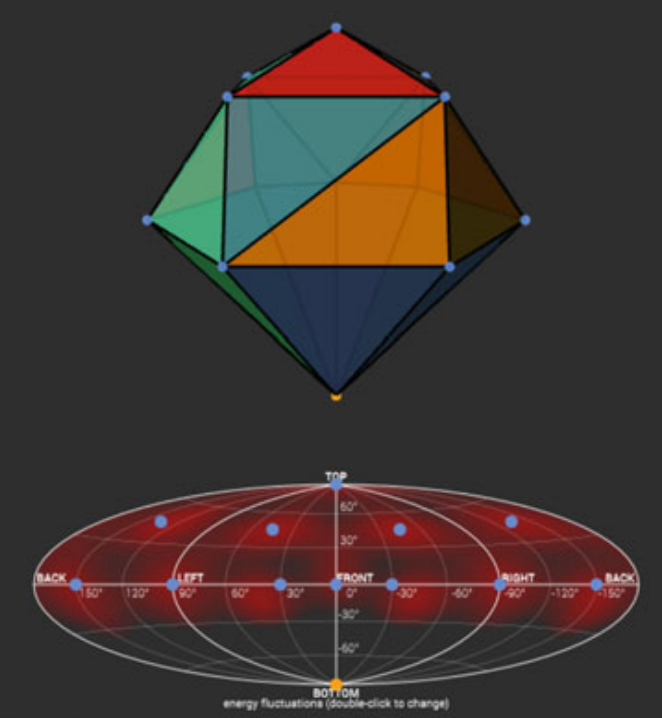
\includegraphics[width=0.4\textwidth]{aufbau/plots/speaker_pos_prod_studio.png}
  \caption{Visualisierung der Lautsprecheranordnung im Produktionsstudio des IEM \protect\footnotemark}
  \label{fig:aufb:prodstud}
\end{figure}

\footnotetext{Quelle: \cite{ambi-book}}

Im Falle unseres Hörversuchs muss unbedingt angemerkt werden, dass der mittige Lautsprecher im Horizontalen Ring, direkt vor der Versuchsperson, fehlte. Dadurch wurde Panning in frontaler Richtung sehr viel hörbarerer sprunghaft. Da dieses Verhalten bei allen Algorithmen und für alle Versuchspersonen gleich war, wurde der Hörversuch jedoch trotzdem durchgeführt.

Tabelle zeigt die Richtungen der einzelnen Lautsprecher, nummeriert wie sie in allen Presets von Ambisonics-Plugins am Studiorechner referenziert werden.



\paragraph{Versuchsinterface}
Um die Antworten der Versuchspersonen auszuwerten wurde eine MUSHRA-Anwendung eingesetzt (MUltiple Stimuli with Hidden Reference and Anchor). Diese Anwendung wird über eine \textit{.json}-Datei konfiguriert und kann als Steuerung für die Reaper DAW verwendet werden. Die Anwendung teilt Zeitspur der DAW in "scenes" auf. Unterschiedliche Klangbeispiele werden daher als Marker zeitlich aufgeteilt. Die verglichenen Algorithmen werden als Fader in der DAW gesteuert. Schaltet man in MUSHRA einen Algorithmus ein, um ihn hörbar zu machen, wird also ein Regler einer Spur in Reaper auf 0dB aufgezogen. Die FOA-Referenz wurde in den getesteten Algorithmen ebenfalls inkludiert.

Die MUSHRA-Anwendung zeigt alle Algorithmen in randomisierter Reihenfolge auf einer eigenen Seite für jede Szene (Klangbeispiel) dar. Dadurch kann die Versuchsperson bei einem Hörbeispiel alle möglichen Algorithmen vergleichen und mit Schiebereglern auf einer kontinuierlichen Skala bewerten. Wenn eine Szene bewertet wurde kann die Versuchsperson zur nächsten wechseln.